%!TEX TS-program = pdflatex
%!TEX encoding = UTF-8 Unicode
%!TEX spellcheck = English (Aspell)

\documentclass[11pt]{article}
\usepackage{../../jeffe,../../handout,graphicx}

\def\Cdot{\mathbin{\text{\normalfont \textbullet}}}
\def\Sym#1{\texttt{\color{BrickRed}#1}}
\def\ForceSym#1{\setbox0\hbox{A}\hbox to \wd0{\hss #1\hss}}
\def\Blank{\ForceSym{$\square$}}

% =========================================================
\begin{document}

\headers{CSCI 432/532}{Problem Session 9a}{Spring 2026}

\noindent
Proving that a problem $X$ is {NP}-hard requires several steps:
\begin{itemize}
\item
Choose a problem $Y$ that you already know is {NP}-hard (because we told you so in class).
\item
Describe an algorithm to solve $Y$, using an algorithm for $X$ as a subroutine.  Typically this algorithm has the following form:  Given an instance of $Y$, transform it into an instance of~$X$, and then call the magic black-box algorithm for $X$.
\item
\EMPH{Prove} that your algorithm is correct.  This always requires two separate steps, which are usually of the following form:
\begin{itemize}
\item
\EMPH{Prove} that your algorithm transforms “good” instances of $Y$ into “good” instances of~$X$.
\item
\EMPH{Prove} that your algorithm transforms “bad” instances of $Y$ into “bad” instances of $X$.  Equivalently:  Prove that if your transformation produces a “good” instance of $X$, then it was given a “good” instance of $Y$.
\end{itemize}
\item
Argue that your algorithm for $Y$ runs in polynomial time.  (This is usually trivial.)
\end{itemize}

\hrule
\vspace{12pt}

\begin{enumerate}
\parindent 1.5em \itemsep 4ex

\item
Recall the following \textsc{$k$Color} problem:  Given an undirected graph $G$, can its vertices be colored with $k$ colors, so that every edge touches vertices with two different colors?

\begin{enumerate}
\item
Describe a direct polynomial-time reduction from \textsc{3Color} to \textsc{4Color}. 
\item
Prove that \textsc{$k$Color} problem is {NP}-hard for any $k \ge 3$.
\end{enumerate}

\item
A \emph{Hamiltonian cycle} in a graph $G$ is a cycle that goes through every vertex of $G$ exactly once.  Deciding whether an arbitrary graph contains a Hamiltonian cycle is {NP}-hard.

A \EMPH{tonian cycle} in a graph $G$ is a cycle that goes through at least \emph{half} of the vertices of~$G$.
Prove that deciding whether a graph contains a tonian cycle is {NP}-hard.

\item
Let $G$ be an undirected graph with weighted edges.  A  Hamiltonian cycle in $G$ is \EMPH{heavy} if the total weight of edges in the cycle is at least half of the total weight of all edges in $G$.  Prove that deciding whether a graph contains a heavy Hamiltonian cycle is {NP}-hard.

\begin{center}\footnotesize\sffamily
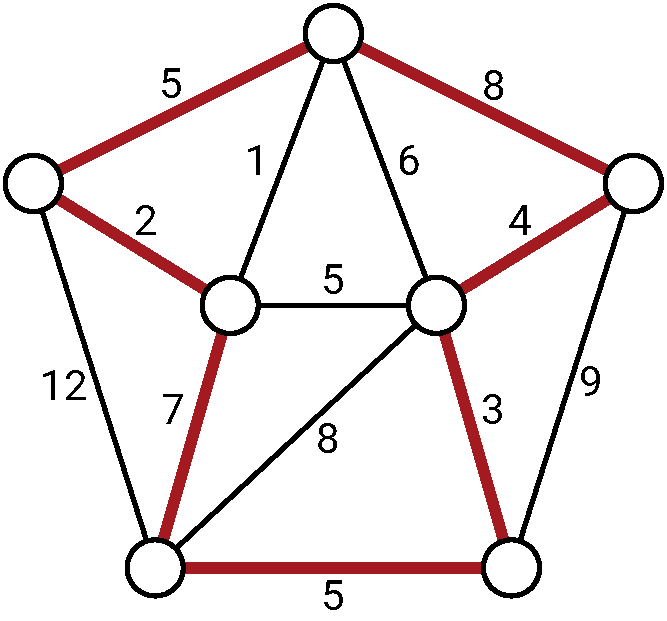
\includegraphics[scale=0.4]{../Fig/heavyham}\\
A heavy Hamiltonian cycle.  The cycle has total weight 34; the graph has total weight 67.
\end{center}

\end{enumerate}



\end{document}